\chapter{Initial model}
We will make 2 models where the output of one is the input of the other. The first of these models determines the probability of a sample being either methylated or unmethylated. The second model determines based on those probabilities whether it comes from someone with a tumor or without. 
\section{Methylation  classification model}
This is the first proper step in the creation of the model that should be able to predict whether a given person may have a tumor based on blood analysis.

This first step is the creation of a \textit{binary classification model} to determine whether we are looking at a methylated or unmethylated region. We decided that a \textit{logistic regression} using \textit{L1 normalization (LASSO)} should be a good classifier. We used the same PCA data as in previous chapters to train and test the model. In addition we also used cross validation to minimize the chance of overfitting. We decided that training on even and testing on odd should be adequate. Using \textit{SKlearn} we created the following code to create, train and test the model.
\begin{python}
pipe = make_pipeline(LogisticRegression(penalty='l1', solver='liblinear',max_iter=1000))
    param_grid = {
        'logisticregression__C': np.logspace(-3, 3, 1000)  # Values for regularization parameter C
    }

    grid_search = GridSearchCV(pipe, param_grid, cv=10, n_jobs=-1)
    grid_search.fit(X_train, y_train)



    best_model = grid_search.best_estimator_

    train_accuracy = best_model.score(X_train, y_train)
    test_accuracy = best_model.score(X_test, y_test)
    num_selected_variables = np.sum(best_model.named_steps['logisticregression'].coef_ != 0)
\end{python}
We end up with 100\% accuracy in our prediction of methylated and unmethylated, while this is regularly a red flag we do not find it too surprising as even just with 2 principal components we could almost separate methylated and unmethylated into 2 distinct clusters. Here is a graph showing the values of the coefficients for the different principal components.

With a good classifier for methylated and unmethylated set up we moved on to the next model.
\section{Tumor classification}
In the previous model we trained the model on only healthy sample, now we try too fit all samples including the the tumor samples. The idea would be that we would have a lower certainty in our methylation classification when using a tumor sample, and that we should be able to find an ideal percentage certainty for a cutoff to do this we used ROC curves
\section{ROC curve}
We used standard SKlearn ROC curve functions to make the ROC curve, we specifically used the following setup
\begin{python}
fpr, tpr, _ = metrics.roc_curve(y, y_scores)
AUC = metrics.roc_auc_score(y, y_scores)
\end{python}
This allowed us to create ROC curves like this
\begin{figure}[H]
	\centering
	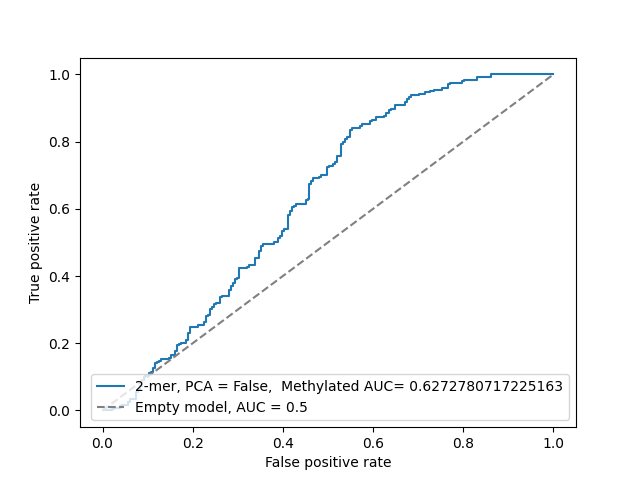
\includegraphics[width=0.7\linewidth]{../../figures/methylation_model/ROC/2-mer, PCA = False Methylated.png}
	\caption{A ROC curve of the methylated 2-mers without PCA}
	\label{fig:allhealthy2}
\end{figure}
The other models can be found in the figures folder however, they all have around 0.4 - 0.6 AUC. This is not ideal, though it does show that there is a possibility of potentially using a different method to predict cancer.
Thus, we decided that maybe we should cut out the middle step of determining methylation and instead go straight to predicting cancer. This new model will be called the "Straight model".
\newpage
\chapter{The straight model}
This model was generally the same as the initial model just with a few key differences were as follows. Instead of training and testing on half of the healthy respectively we were now able to train and test on half of all samples for all regions. Thereby increasing the data for the model. The other being that our new targets for training the model being cancer/noncancer instead of methylation. 
Using this we were able to create the following ROC curves using the same method as before giving us these results.
\begin{figure}[H]
	\centering
	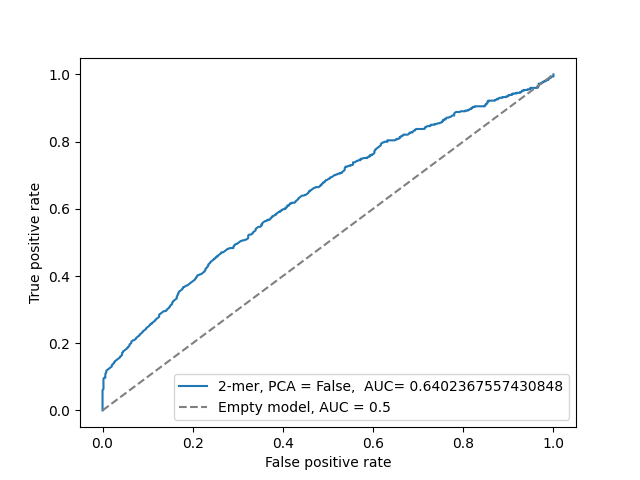
\includegraphics[width=0.7\linewidth]{../../figures/straight_model/ROC/2-mer, PCA = False.png}
	\caption{A ROC curve of the methylated 2-mers without PCA}
	\label{fig:allhealthy2}
\end{figure}
As you can see not much of an improvement though it does seem to be more consistent than our previous method, giving us only AUC above 0.5. 